\documentclass[../Thesis_AHoecherl.tex]{subfiles}

\begin{document}
    \section{Instruments, pricing and market data}\label{Instruments, pricing and market data}
    For the analysis whose results are presented in chapter \ref{sec:Results}, a small but diverse set of financial instruments is required. Due to the structure of the \gls{ISDA SIMM} and the \gls{SA-CCR} model the set of financial instruments should meet the following criteria:

    \begin{enumerate}
        \item The instruments should range across multiple asset classes
        \item Non-linear instruments should be included
        \item The instruments should range across multiple currencies
        \item The instruments should be commonly traded as bilateral, uncleared derivatives to be relevant for \gls{ISDA SIMM} \label{uncleared}
        \item Pricing and sensitivity calculation should be possible without implementation of simulation approaches \label{easy_to_price}
        \item Inferring market data objects required for pricing from market quotes of traded instruments must be simple \label{link_to_market_quotes}   
    \end{enumerate}
    
    Items \ref{uncleared} and \ref{easy_to_price} of the above list are slightly conflicting. Bilaterally traded derivatives are usually more complex than cleared derivatives. Due to this increased complexity many of them have to be priced with a Monte Carlo simulation since an analytical solution is not possible.

    Item \ref{link_to_market_quotes} rises from the requirement of the \gls{ISDA SIMM} model to calculate all sensitivities against market quotes. This means for example, that interest rate sensitivities mustn't be calculated with regard to a movement of the interest rate curve used as a pricing input but with regard to the price of the traded instrument that is used to build the interest rate curve in the first place. In the case of interest rate curves the process to build an interest rate curve is commonly referred to as \emph{bootstrapping} and has to be performed again whenever a sensitivity is calculated to be compliant with \gls{ISDA SIMM}. Designing a pricing framework that can handle this required interdependence of market quotes, market data objects such as curves and priced instruments is a steep task even for deceptively simple instruments such as plain vanilla interest rate swaps. For this reason the implementation is based on QuantLib \cite{QuantLib} which offers an excellent and proven framework to monitor these interdepencies with ease.

    Careful consideration of the criteria listed above and the available market data lead to the following set of financial instruments that will be used for analysis:

    \begin{itemize}
        \item Overnight indexed swaps
        \item Fixed-float interest rate swaps
        \item European equity options
        \item Swaptions
    \end{itemize}

    In the following, we will outline how these instruments are priced, what market data is used for this and how \gls{ISDA SIMM} compliant sensitivities are calculated for each instrument.

    The instruments just serve as a means to perform the analysis of the topics on which the thesis is focused which are the \gls{SA-CCR} model, margining and risk measure allocation.
    Accordingly, pricing algorithms and required market data have been chosen rather pragmatically and do not claim to represent the currently established state-of-the-art in pricing these derivatives.
    In line with the focus of the thesis the following explanations on derivative pricing, market data and sensitivity calculation are kept brief.  

    A basic familiarity of the reader with interest rate derivative markets and equity derivative markets is assumed. 
    A basic introduction to both may be found in \cite{hull2009options}. A comprehensive approach to interest rate derivative markets may be found in \cite{brigo2007interest} or \cite{andersen2010interest}.

    \subsection{Overnight indexed swaps}\label{sec:Overnight indexed swap}

    An overnight indexed swap (\gls{OIS}) is a fixed-float swap whose floating leg underlying are the daily fixings of an overnight index.
    It can be priced using the so called \gls{OIS}-curve, whose construction will be discussed below.
    Usually, only a single \gls{OIS} curve exists per currency which is used both as a forward curve for estimating future cashflows on the floating leg of an OIS swap and as a \emph{'risk free'} discounting curve for all cash flows of the given currency.

    The net present value (\gls{NPV}) of an \gls{OIS} may be calculated like that of any other swap by estimating future cashflows of the floating leg with the appropriate interest rate curve and discounting all cashflows of the swap with the currencies' discount curve.
    Accordingly, an \gls{OIS} Swap may be priced using only the \gls{OIS} curve of the swaps currency.

    Since the \gls{OIS} curve also serves as the discount curve it does not require any other interest rate curve to be constructed. 
    For the purpose of this thesis, EUR and USD \gls{OIS} curves were built from the par rates of \gls{OIS} swaps as they were quoted on the 10th of May 2019.\footnote{To build an arbitrage free \gls{OIS} curve especially the short end should be based on more than just \gls{OIS} quotes as is for example pointed out in \cite{ametrano2013everything} or \cite{brugger2018valuation}. However, for this thesis higher accuracy in curve construction was not required.}
    Conveniently, QuantLib does offer a built in functionality to infer an \gls{OIS} curve from quoted \gls{OIS} par rates, namely ''OISRateHelper''. Essentially, the \gls{OIS} par curve is built by interpolating between the quotes.
    This par curve may then be transformed into other interest curve representations such as a zero curve, forward curve or a discount curve under the assumptions of a single curve universe. How this can be done is e.g. pointed out in \cite[Chapter 4]{hull2009options}.

    An \gls{OIS} changes its \gls{NPV}, if the \gls{OIS} curve that it used to price it moves.
    This delta sensitivity against points on the \gls{OIS} curve is the basis for the \gls{ISDA SIMM} calculation of an \gls{OIS}.
    \gls{ISDA SIMM} requires interest rate delta sensitivities of an \gls{OIS} to be calculated as a finite difference against movements of the quoted market par rates used to build the \gls{OIS}-curve in the first place. 
    This means that delta sensitivities of an \gls{OIS} are calculated by raising a market quote that was used to build the \gls{OIS}-curve by one basis point, rebuilding the \gls{OIS}-curve as described above and repricing the \gls{OIS} for which the delta is being calculated.
    A definition of \gls{ISDA SIMM} compliant interest rate deltas may be found in \cite[Point 22]{SIMM} and \cite[Section 2.2]{RiskDataStandard}.
    
    Additionally, an FX delta needs to be calculated which is used if the trade currency does not coincide with the \gls{ISDA SIMM} calculation currency that was agreed upon in the \gls{CSA}. This delta may be approximated as $0.01 * NPV$ if the trades underlying is not an exchange rate \cite[Section 2.7]{RiskDataStandard}.

    In fact, such an FX delta is required for all of the following derivatives and as none of them are FX derivatives can always be calculated as $0.01 * NPV$.

    \subsection{Interest rate swaps}

    In a narrow definition, interest rate swaps or \gls{IRS} are swaps of a single currency, which have a floating and a fixed leg and whose floating leg references not an \gls{OIS} index but rather an index of a larger tenor such as the six month \gls{EURIBOR} index.

    For this thesis, \gls{IRS} on the six months \gls{EURIBOR} and three month USD \gls{LIBOR} index are set up for analysis.
    These tenors have been chosen as they are the reference tenors for their respective currencies. 
    This indicates that \gls{IRS} on this tenor are very liquid whereas other tenors are rather traded through float-float basis swaps between the reference tenor and another tenor of the same currency.

    As for an \gls{OIS}, an \gls{IRS} is priced by estimating future payments of the floating leg through the tenor curve and then discounting all cash flows whether they are estimated or fixed.
    However, unlike the \gls{OIS} the curve used for forecasting future payments and discounting generally does not coincide.

    The presence of multiple interest rate curves per currency, i.e. a multi-curve universe has become widely accepted since the financial crisis of 2008 raised awareness for the credit risks associated with interbank lending.
    This has complicated interest rate curve construction and made a bootstrapping approach in which the interest rate curves of a currency are built up incrementally starting with the \gls{OIS} curve necessary.
    The bootstrapping of a multi curve environment is a rather intricate process and is described in detail for example in \cite{ametrano2013everything} and \cite{brugger2018valuation}.
    However, for the purpose of this thesis, it is sufficient to know that under bootstrapping, the zero rate curve of a reference Libor curve such as the 6M \gls{EURIBOR} curve is dependent on both, the par rates quoted for 6M \gls{EURIBOR} \gls{IRS}\footnote{To be exact, not only interest rate swaps but also forward rate agreements on the 3M USD \gls{LIBOR} and 6M \gls{EURIBOR} were used. Again market data as observed on the 10th of May 2019 is used for all calculations presented in section \ref{sec:Results}.} as well as the par rates quoted for \gls{OIS}-curve of the same currency.

    To calculate an \gls{ISDA SIMM} compliant sensitivity against a specific quoted par rate that was used to construct the \gls{OIS} or tenor curve is shifted, the bootstrapping is repeated to yield the \gls{OIS} curve and the forward curve of the underlying interest rate curve and the \gls{IRS} is repriced.    

    \subsection{European Equity Options}\label{sec:European Equity Options}

    For the purpose of this thesis, European equity options are priced analytically with a Black Scholes model as it is for example introduced in \cite[Chapter 14]{hull2009options}. The model was originally published in \cite{black1973pricing}.

    To do so, QuantLib offers the \emph{BlackScholesProcess} class which can be constructed from the current spot value of an equity, a discount curve of the relevant currency and a volatility surface of implied volatilities with option maturities in one dimension and option strikes in the other.

    As a discount curve the \gls{OIS} curve introduced in \ref{sec:Overnight indexed swap} is used.
    On the other hand, equity spot and volatility surface dummy data was fabricated for two equities with the volatility surfaces being flat.
    This fabricated data is sufficient for the purpose of this thesis as its structure allows for an easy calculation of \gls{ISDA SIMM} compliant sensitivities\footnote{The used constructed volatility surface has for example exactly the maturity vertices that \gls{ISDA SIMM} expects without further interpolation being necessary.} and for the analysis conducted for section \ref{sec:Results} it is irrelevant whether the used market data has actually been observed or has been fabricated.

    The relationship between the market data from which a volatility surface is built and the volatility surface itself is straight forward.
    Implied volatilities of options are directly quoted by the market and can be put on a grid based on the option maturity and strike of the option for which they are quoted.
    Afterwards, the volatility surface is created by simply interpolating between these points. For this thesis a bilinear interpolation and extrapolation was chosen.

    When pricing a European equity option the relevant risk free interest rate can be identified by retrieving the zero rate for the option maturity from the \gls{OIS} curve of the currency in which the equity is traded.
    Afterwards, an equity volatility can be retrieved from the volatility surface by interpolating the implied volatility for the strike and option maturity of the option that should be priced.
    These two values can then be used as the risk free rate and equity volatility in the call or put Black Scholes formula to price the option.

    According to \gls{ISDA SIMM}, an equity option has equity delta, equity vega, interest rate delta and FX delta risk. The FX delta risk is calculated in the same way as described for an \gls{OIS} in section \ref{sec:Overnight indexed swap}.
    An interest rate delta sensitivity is calculated by shifting an \gls{OIS}\gls{OIS} par rate, rebuilding the \gls{OIS} curve as pointed out in section \ref{sec:Overnight indexed swap} and afterwards inferring a new risk free rate from this rebuilt \gls{OIS} curve for a new valuation under the Black Scholes model.
    An \gls{ISDA SIMM} compliant equity delta is calculated by increasing the spot price of the underlying equity by one percent and repricing the option under the Black Scholes model.
    Finally, \gls{ISDA SIMM} compliant equity volatility sensitivities, i.e. vegas, are calculated by increasing all quoted implied volatilities that share a common option maturity by $0.01$, interpolating again to retrieve a new volatility surface and proceed with repricing the option as described above.

    Rules on how equity sensitivities and equity volatility sensitivities have to be calculated for the purpose of \gls{ISDA SIMM} are defined under \cite[Section 2.5 and 2.8]{RiskDataStandard} and \cite[Points 21, 26 and section C.3]{SIMM}.

    \subsection{Swaptions}

    For the purpose of this thesis the primary approach to pricing swaptions is use of the Black model \cite{black1976pricing}. This model was originally developed for European options on commodity or equity future contracts and is very similar to the Black-Scholes model but models the development of a forward price instead of spot prices.
    Both, the Black-Scholes model and Black model models assume that return follow a log-normal distribution.
    If forward rates of interest rates become negative, the Black model can therefore not be used since log return of negative values can't be calculated.
    In these cases, an alternative model by Bachelier \cite{bachelier1990theorie} which assumes the forward rate to follow a normal process can be used.
    The application of the Bachelier model for swaption pricing is e.g. presented in \cite{floc2016fast}.

    Both the Black model and the Bachelier model require the volatility of the underlying as in input. Similar to what was described for the Black-Scholes model in \ref{sec:European Equity Options} these can be captured in a volatility surface or, depending of the granularity of used input instruments, a structure of even higher dimension.
    It is important to note that the implied volatilities used for either the Bachelier or the Black model need to be inferred from option prices using the respective model.
    One cannot, for example, calculate the implied volatility of a swaption with a Black model and use the resulting number afterwards in the Bachelier formula.
    The Chicago Mercantile Exchange publishes both the implied volatilities under the normal and under the log-normal model of swaptions on their website
    \footnote{ftp://ftp.cmegroup.com/irs/}.

    For this thesis swaptions reference swaps on either the six month \gls{EURIBOR} or the three month USD \gls{LIBOR}.
    Market data of the 10th of May 2019 has been used, a time at which the interest rates between the two currencies were quite different, with the \gls{EURIBOR} 6M zero curve being partially negative as can be seen in figure \ref{fig:EURIBOR and LIBOR forward curve}\footnote{This figure is produced in Appendix \ref{usd-libor-and-euribor-zero-curves}.}.

    \begin{figure}
        \centering
        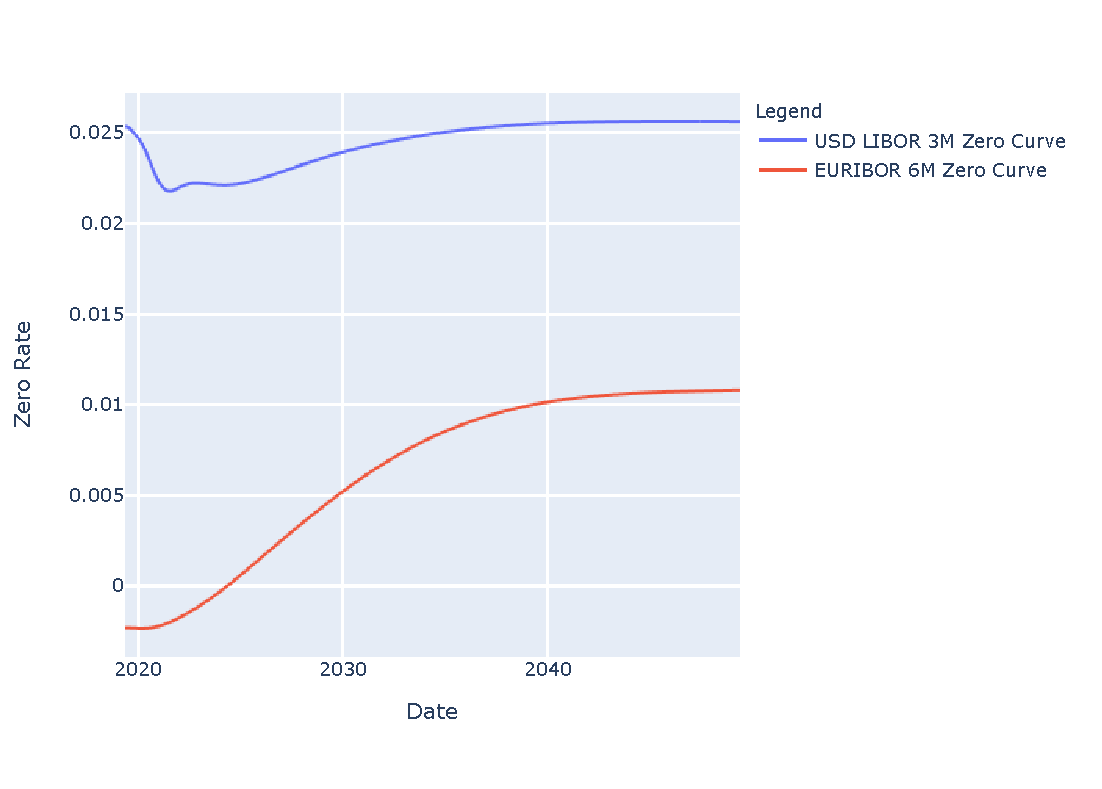
\includegraphics{Graphics/EURIBOR_and_LIBOR_curve.pdf}
        \caption[EURIBOR 6M and USD LIBOR 3M zero curve]{\gls{EURIBOR} 6M and USD \gls{LIBOR} 3M zero curve on the 10th of May 2019. It can be seen that the USD \gls{LIBOR} zero rate is constantly well above zero percent while the zero rate of the \gls{EURIBOR} remains negative for the first couple of years.}
        \label{fig:EURIBOR and LIBOR forward curve}
    \end{figure}

    For this reason, swaptions on the \gls{EURIBOR} 6M index are priced with a Bachelier model while swaptions on the USD \gls{LIBOR} 3M index are priced with a Black model, both of which offer analytical solutions to price a swaption.

    In similar fashion to Black-Scholes pricing of equity options the swaption is priced by first interpolating a volatility that matches the option maturity and swap maturity of the priced swaption\footnote{We are working with a two dimensional swaption volatility surface which only contains the implied volatilities of at-the-money swaptions and does not differentiate based on moneyness of the option. This is in line with the grid for interest rate vegas that the \gls{ISDA SIMM} model defines in \cite[Section 2.8]{RiskDataStandard} and \cite[Point 10]{SIMM}} and inferring a the forward rate from the interest rate curve that matches the start and end-point of the underlying swap.
    This forward rate and volatility are then plugged into the respective Black or Bachelier formula for a European Call if the underlying is a receiver swap or of a European Put if the underlying is a payer swap.

    Calculation of \gls{ISDA SIMM} compliant sensitivities happens in same way as for the previous products.
    To yield interest rate delta sensitivities par quotes used to build either the \gls{OIS} or LIBOR or \gls{EURIBOR} curve are shifted, and bootstrapping is re-executed to yield a new forward interest rate curve.
    From this forward curve the relevant forward rate of the underlying swap is inferred, plugged into the Bachelier of Black pricing formula and the swaption is repriced to yield the delta sensitivity against the initially shifted par quote.

    Interest rate vega sensitivities against the volatility are calculated in the same way as those of an European equity option.
    They are calculated by increasing all quoted implied volatilities that share a common option maturity by $0.01$, interpolating again to retrieve a new volatility surface and proceed with repricing the swaption as described above.

    Finally, FX sensitivities are calculated again as one percent of the \gls{NPV} of the swaption as was also the case for the other instruments.



\end{document}